We conduct our study in a large scale open source software system to distinguish Defect Debt and Bugs. First, we analyze the history of issues in the system, and then we suggest a definition to Defect Debt and to Bugs. Based on this definition we quantify  both on them per release. Second, we analyze the evolution of Defect Debt to understand its impact on future feature addition. Third, based on our metrics we propose a model to Defect Debt.

\vspace{3mm}
\noindent\rqi
\vspace{3mm}

\noindent\textbf{Motivation:} Technical Debt is a broad concept and can be classified in many subcategories (e.g., Design Debt, Documentation Debt, Defect Debt). However, these subcategories may not have a clear definition making difficult to distinguish them to already know terms (i.e, Defect Debt and Bugs). Answering this research question, will provide us a way to identify and quantify Defect Debt. 

\vspace{1mm}
\noindent\textbf{Approach:} To identify Defect Debt we first, mine the project issuer tracker to extract the bug reports. Then, we link the bug report to its respective software release using the reported date. 

Second, we extract the commits from the source code repository. In some projects like Google Chrome, it is a common practice to add the bug id in the commit message. Based on this knowledge, we use the commit messages to link the commits with bug reports. Regular expressions are the most common way to identify bug id in the commit message. This technique provide us the exact date that the bug was fixed, which is more precise than reeling on the closing date from the bug report. The trade-off of this technique is that is not always possible to find the bug id for each one of the bug reports, or the bug id in the message can be wrong as it is a manual input. Other than that, it is possible to find multiple commits that corresponds to the same bug id, scenario that need further investigation when linking. 

Third, we link the commit to its respective release using commit date. For each defect in our system we have the date that they were reported and the date they were fixed. 

Fourth, we take all reported defects for each one of the releases. Then, we group it based on the release they were fixed. In total we did this process for 26 Chrome releases. We plot the data to visualize the distribution of the defects and draw conclusions. 

\vspace{1mm}
\noindent\textbf{Result:} Analyzing the graphs shown in figure \ref{fig:defect_release_1} we observe that most defects are fixed during the release that they were reported or in the immediately next one. A smaller quantity of defects reported in the current release will remain in the system for a long time, but eventually get fixed. The observed pattern holds for each analyzed version. 

\begin{figure}[thb!]
	\caption{Fix for defects reported in release 1.}
	\label{fig:defect_release_1}
	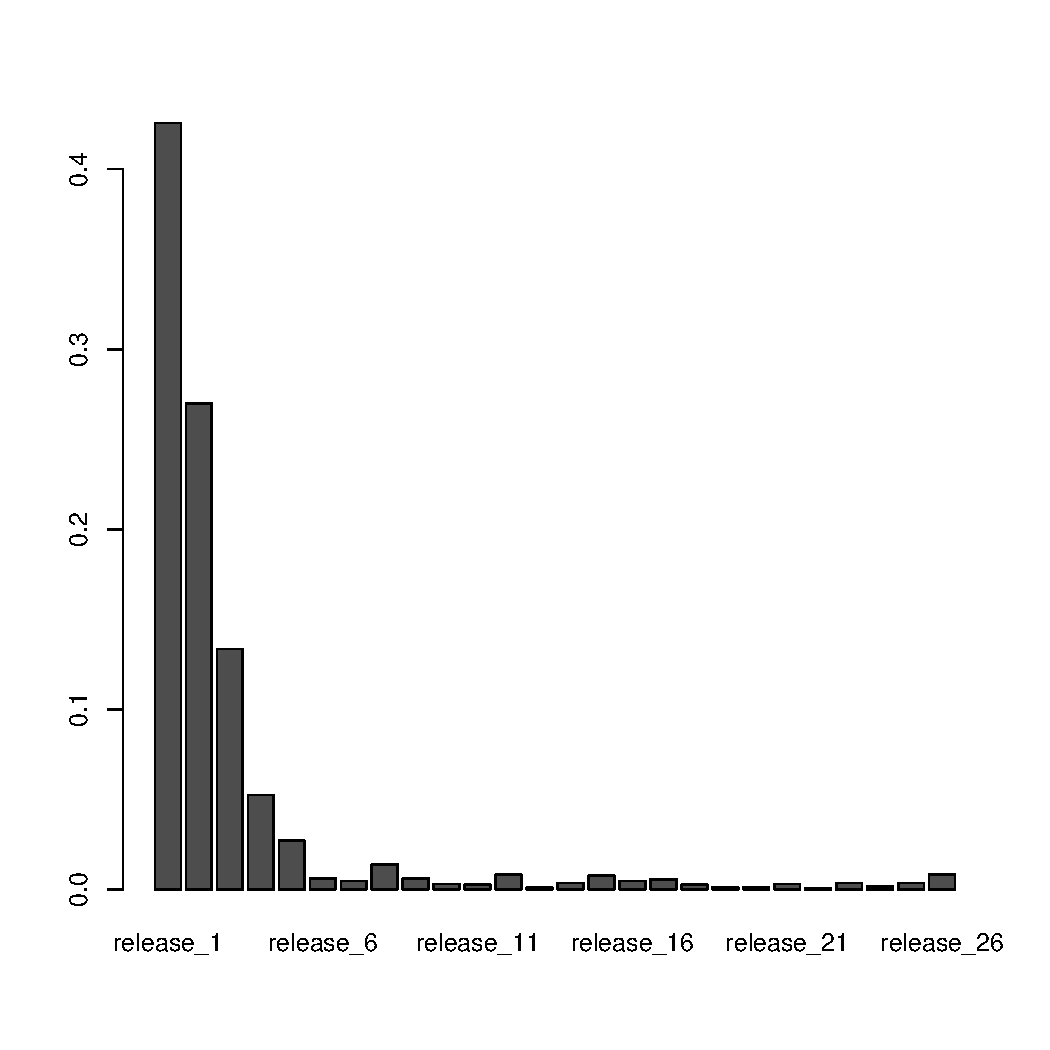
\includegraphics[width=90mm,scale=0.5]{figures/r1}
\end{figure}

\begin{figure}[thb!]
	\caption{Fix for defects reported in release 6.}
	\label{fig:defect_release_6}
	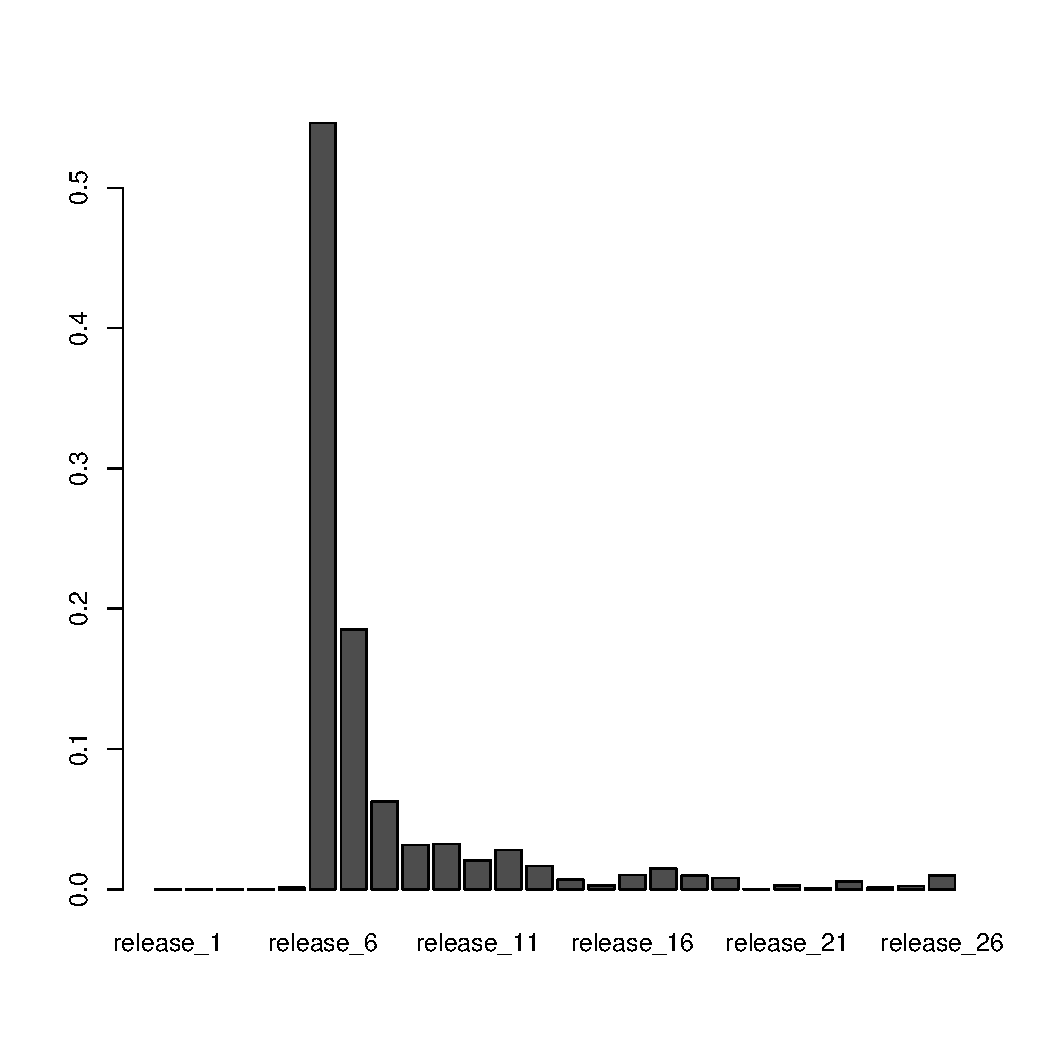
\includegraphics[width=90mm,scale=0.5]{figures/r6}
\end{figure}

In some cases, like shown in figure \ref{fig:defect_release_6} we can observe a reopened bug. (i.e., the same defect has a fix reported in one previous release and in the current release as well). Just based in this argument, we can not say that we were able to identify all reopened bugs in the system. There are different factors that can impact this scenario (e.g., it is possible that a reopened bug has a new bug id in the issuer tracker, and in that case our approach would not identify it as a reopened bug). More investigation is needed in order to explain this phenomena in a satisfactory way. 

Accordingly with our findings, we say that it is possible to distinguish regular Bugs and Defect Debt based on their fix behavior. Bugs are more critical defects and are fixed near to its reported date (i.e., in the same or in the immediately next release), and Defect Debts are defects that lingers in the system for several releases but eventually are fixed. We believe that the fix behavior of the 

There is not hard proof in our study that the reason that Bugs are fixed first than Defect Debt because they are more critical, but based on our experience we argue that tasks in a project are assigned to developers following a priority order. Even considering a open source environment where non-core developers (e.g., an anonymous contributor), could be fixing bugs just because they are easy to fix, previous work by Mockus et al. \cite{mockus2010ICSM} has shown that most of the development activity is done by the core developers of the system.

Based on our findings we quantify the average of Bugs and Defect Debt in the analyzed releases. Considering the reported defects on Chrome has an average of 69.55\% Bugs and 30.44\% of Defect Debt.

\conclusionbox{Bugs are more critical defects, and get fixed in the reported or in the next release. Whereas Defect Debt may linger in the system for a long time, but eventually it get fixed. The average percentage of Bugs is of 69.55\%, and Defect Debt is of 30.44\%}

\vspace{3mm}
\noindent\rqii
\vspace{3mm}

\noindent\textbf{Motivation:} In general Technical debt can bring you short term advantage in trade off maintenance costs in the future. Which means that well managed Defect Debt can be used as a tool to achieve projects goals. That said, we want to how Defect Debt impact the addition of new features in the system. We want to know if the increase of Defect Debt will result in a decrease in feature addition. 

\vspace{1mm}
\noindent\textbf{Approach:} First we track the quantity of open bugs in the system (i.e, Bugs and Defect Debt). It is important to know how many open bugs are present in the system, and understand its distribution in the releases. This way we can visualize the system "health" in terms of defect. To calculate the total number of open bugs of the first release, we subtract the number of fixed bugs from the number of reported bugs the remainder is the number of open bugs of the release. All the subsequents releases have to take into consideration the number of open bugs from the previous release. The formula to calculate open bugs is:

\begin{center}
	$Open bugs=  Reported - Fixed + Last Release OpenBugs$
\end{center}

Second, we extract the number of  Defect Debt from the system. To understand how Defect Debt will impact the number of feature addition we have to collect the total number of Defect Debt per release. We define Defect Debt as a defect that was reported more than 2 releases from the current release being analyzed. We say that a Defect Debt belongs to a release when the fix for the Defect Debt is commited in the release.
 
Third, we label all the commits and group them by release. We use a tool that classify the intention of a commit based on the message that the developer post when he/she is done with the task. A label is one of the possible classifications that this tool provides and, we are interested in all commits that have the label `Feature Addition'.   

Fourth, we compare the distribution of Defect Debt with the distribution of Feature Addition commits. To see the distribution of Defect Debt we group the total number of Defect Debt per release and plot a graph with the result. Then we group the total number of commits labeled as `Feature Addition' per release and plot a graph with the result.

\vspace{1mm}
\noindent\textbf{Result:} We show the number of open bugs in figure \ref{fig:number_of_bugs_releases}. We found that the number of bugs keep increasing as the project gets older. Towards the end of the graph we see a major decrease in the number of open bugs in the system, but this happened as a reflexion of our data. As we get near the end of our data set, we see the effects of the lack of information about future releases. 

\begin{figure}[thb!]
	\caption{Number of open bugs per release}
	\label{fig:number_of_bugs_releases}
	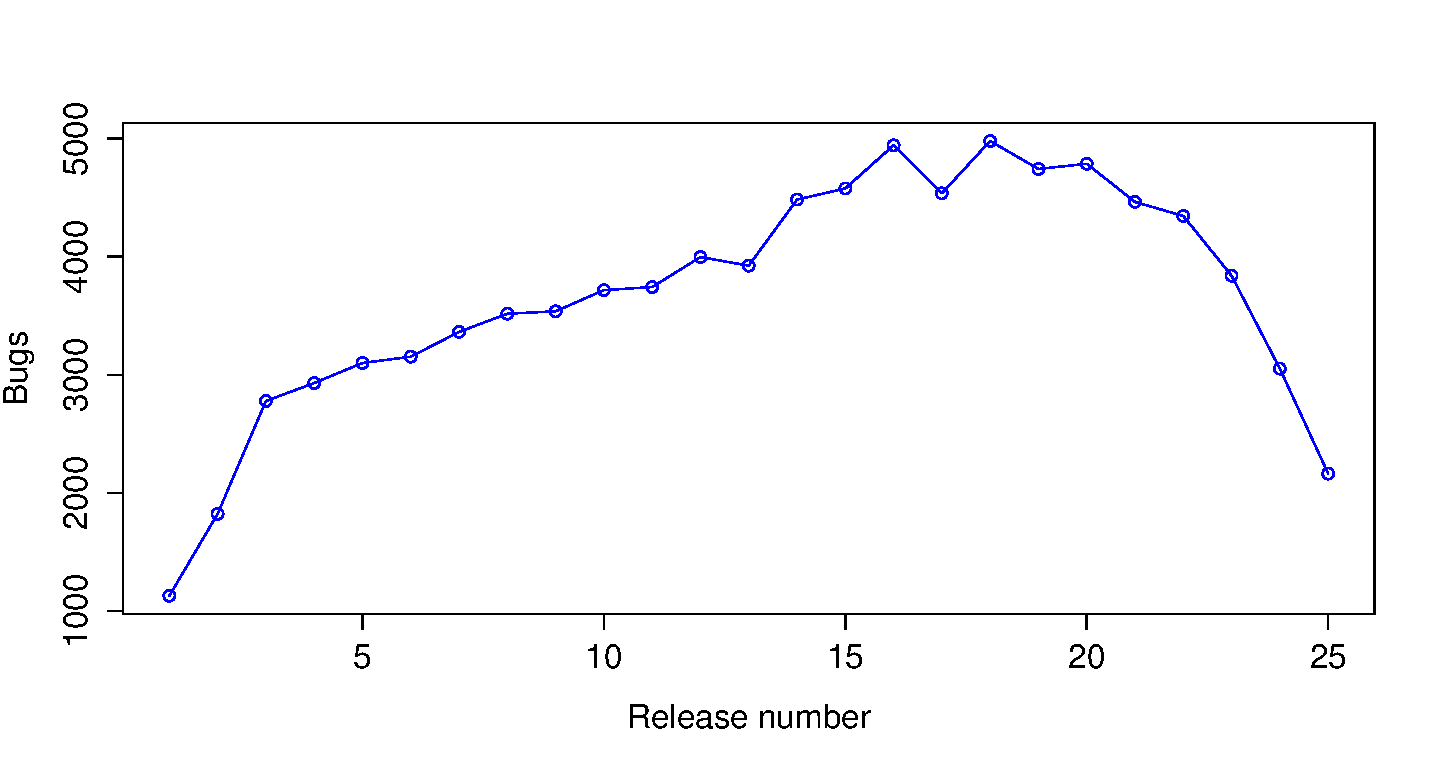
\includegraphics[width=90mm,scale=0.5]{figures/number_of_bugs_releases}
\end{figure}
  
Based on this graph we found that during all releases there was a considerable number of open bugs in the system, and the developers of the project prioritize some fixes other than others. This behavior could mean that the bugs that were not fixed because they were not important. In order to analyze that we extract the distribution of the Defect Debt in figure \ref{fig:technical_debt}. We found that the behavior of Defect Debt is much more volatile. We see growth in peaks, but they are fixed in future versions. That means that they are important enough to be fixed, they just delay the fix until a moment that it is more fit to fix it.

Analyzing the number of `Feature Addition' commits we found that in the first releases has the highest amount of `Feature Addition' commits as shown in figure \ref{fig:feature_addition_releases} . This confirms what we expected to see in the beginning of the development of a product. Surprisingly though is that the number of Defect Debt does not seems to cause a negative impact in the addition of new features. Analyzing both graphs we see that as the number of feature addition increases we have a increase in the number of Defect Debt as well. This lead us to the conclusion that new features brings more Defect Debt to the system and that after some releases they are corrected. We show detailed information about feature addition distribution and Defect Debt distribution in table \ref{tab:feature_addition_badsmell_overview}.

Although the number of Defect Debt have no impact in the number of feature addition, we can not say that Defect does not cause any other kind of impact. In this study we did not take in consideration the number of developers needed to keep adding features or the amount of time necessary to do it. we understand that more analysis is necessary to understand what is the impact that Defect Debt has in the quality of a software project.

\conclusionbox{Based on our study, the number of Defect Debt does not impact directly the number of feature addition in the project. Moreover, the increase of feature addition may increase the number of Defect Debt. The average number commits classified as feature addition in Chrome is of 349.24 per release, whereas average number of Defect Debt found in each release is of 648.52 }

\begin{table}[!hbt]
      \begin{center}
            \caption{Feature addition and Defect Debt overview}
            \label{tab:feature_addition_badsmell_overview}
            \begin{tabular}{l| c c }
            \toprule
            \textbf{Release}  & \textbf{Feature Addition} & \textbf{Defect Debt} \\ \midrule 
              1  & 1046 & 598   \\ 
              2  & 622 & 560    \\ 
              3  & 487 & 1044   \\ 
              4  & 520 & 604    \\ 
              5  & 463 & 800    \\ 
              6  & 185 & 465    \\ 
              7  & 163 & 530    \\ 
              8  & 187 & 582    \\ 
              9  & 148 & 377    \\ 
             10  & 253 & 606    \\ 
             11  & 201 & 427    \\ 
             12  & 313 & 763    \\ 
             13  & 255 & 561    \\ 
             14  & 230 & 561    \\ 
             15  & 315 & 849    \\ 
             16  & 274 & 789    \\ 
             17  & 367 & 876    \\ 
             18  & 354 & 687    \\ 
             19  & 287 & 946    \\ 
             20  & 228 & 738    \\ 
             21  & 398 & 498    \\ 
             22  & 288 & 882    \\ 
             23  & 475 & 438    \\ 
             24  & 394 & 642    \\ 
             25  & 278 & 390    \\ \bottomrule
            \end{tabular}
      \end{center}
\end{table}

\begin{figure}[thb!]
	\caption{Distribution of Defect Debt}
	\label{fig:technical_debt}
	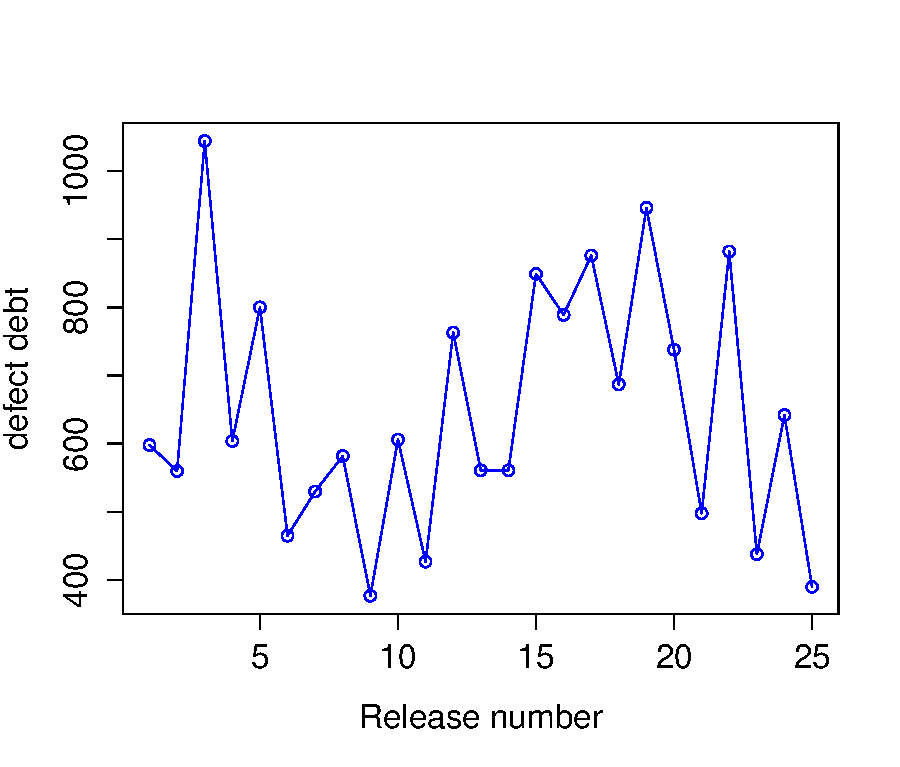
\includegraphics[width=90mm,scale=0.5]{figures/technical_debt}
\end{figure}

\begin{figure}[thb!]
    \caption{Release density evolution}
    \label{fig:feature_addition_releases}
    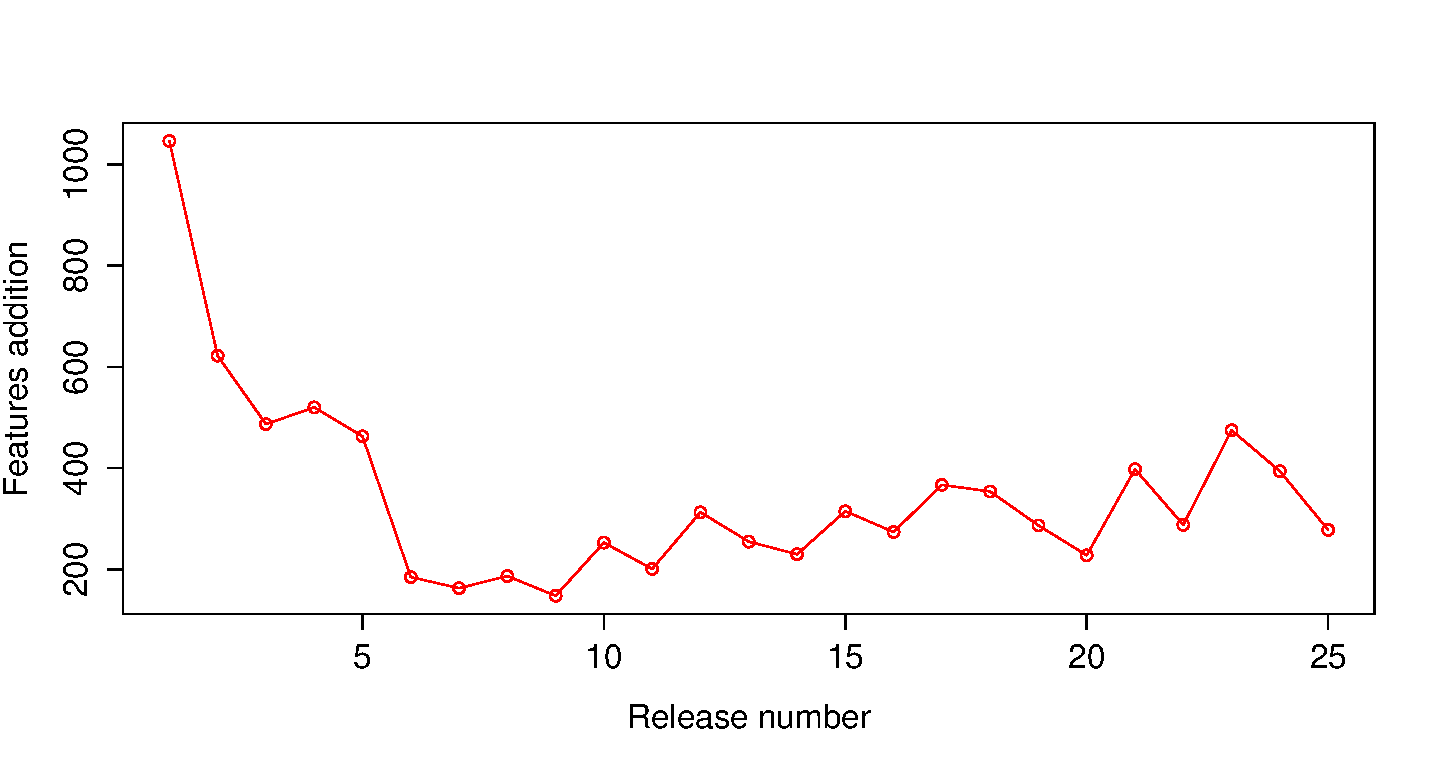
\includegraphics[width=90mm,scale=0.5]{figures/feature_addition_releases}
\end{figure}

\vspace{3mm}
\noindent\rqiii
\vspace{3mm}

\noindent\textbf{Motivation:} We want to know if it is possible to determine what are the important factors when modeling Defect Debt. Answering this question will provide us with more means to effectively manage Defect Debt by knowing before hand that the specific defect will have to be handled in the future carefully to avoid quality impacts based on the factors that are important in the model. 

\vspace{1mm}
\noindent\textbf{Approach:} First we selected  of metrics that we believed that would be good indicators of Defect Debt. In our data base we prepared the following metrics per release: number of corrective commits, number of feature addition commits, number of merge commits, number of non function commits, number of perfective commits, number of preventative commits, number of non classified commits, total number of churn, total number of developers, difference of developers from previous release, project complexity, lines of code, number of comments in the bug report, total number of bug fixes and bug reported close to the next release.

Second, we run the analysis in Understand, and build our own script to extracted data using the API. We extract lines of code and complexity of each release using Understand. We process 17 tags of Chrome in this tool creating one database for each tag. The oldest tag that we were able to retrieve from Chrome in this experiment was the tag 10.0.648.127. We cloned the git repository using the repository provided in GitHub \footnote{https://chromium.googlesource.com/chromium/src}. To create our model we just consider tags that we can get all the selected metrics, which means tags ranging to version 10.0.648.127 to 25.0.1364.97.

Third, we import the data into RStudio. RStudio is a tool to the statical analysis using the programming language R. For each one of the metrics that we collect we checked their data distribution. We do that using skewness and kurtosis both are commands from the library `e1071' that can be imported into RStudio. Skewness is used to verify if the data is skewed to the left or to the right in the x axis. The value returned from this function should be close to zero, which means that your data is normally distributed. Kurtosis follows the same principle but is used to check the data distribution in the y axis. After running these commands we apply the log function to the following factors in order to normalize the data: number non functional commits, difference of developers from previous release and number of comments in the bug report. 

Fourth we do the correlation of the factors. and test the results of the correlation.

Fifth, we build the model and do the vif function to verify the factors in the model that are measuring the same thing. 
 
\vspace{1mm}
\noindent\textbf{Result:}

\todo{table with correlation}
\todo{explain the model}
\todo{table with all the results}